\section{Modelos}

\subsection{Comparación visual de los árboles}
El ajuste mediante \texttt{GridSearch} produce un árbol más \textbf{compacto} y, por tanto, \textbf{más explicable} (menos profundidad y reglas), manteniendo o mejorando ligeramente la precisión respecto al baseline. A continuación se muestran por separado ambos diagramas con la misma profundidad visualizada para facilitar la lectura.

\begin{figure}[h]
  \centering
  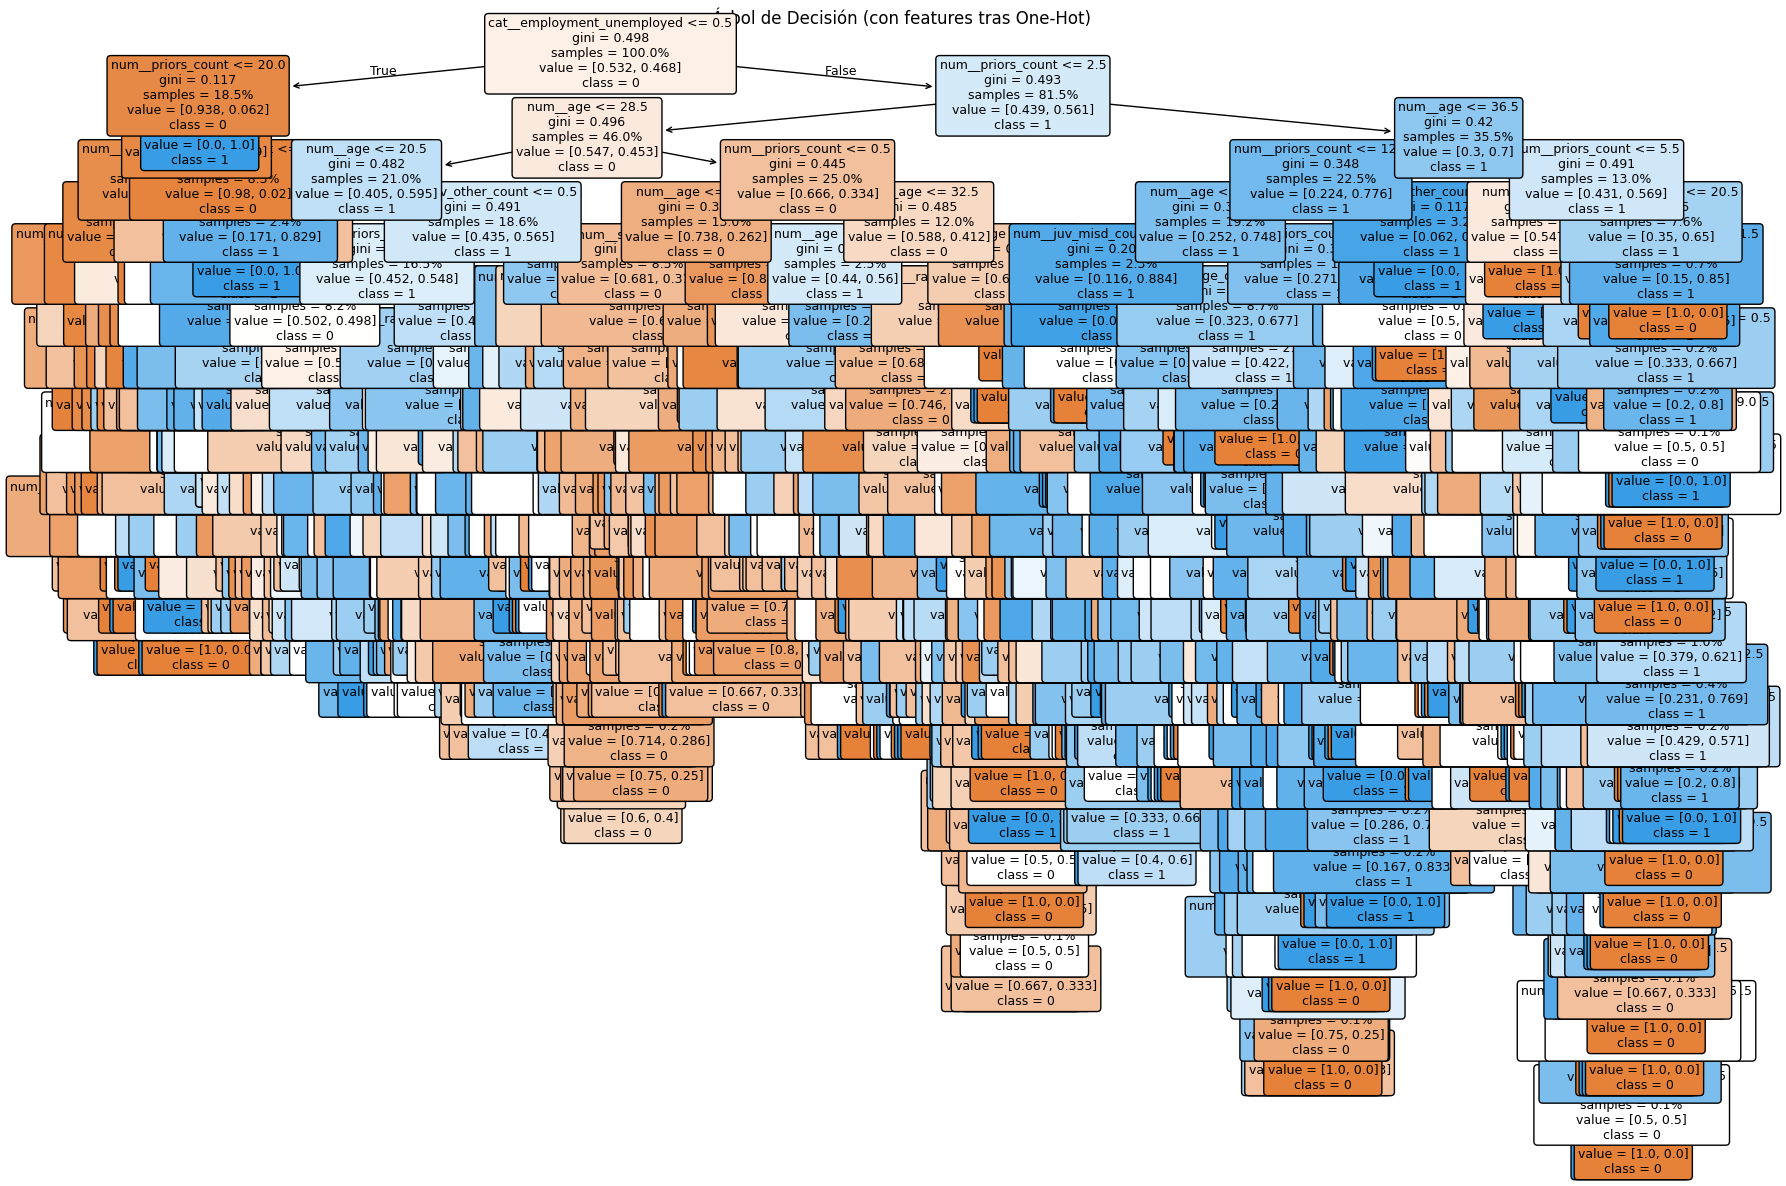
\includegraphics[width=0.92\linewidth]{figures/decision_tree_baseline_depth.png}
  \caption{Decision Tree (baseline), profundidad visualizada = 3.}
  \label{fig:tree-base}
\end{figure}

\begin{figure}[h]
  \centering
  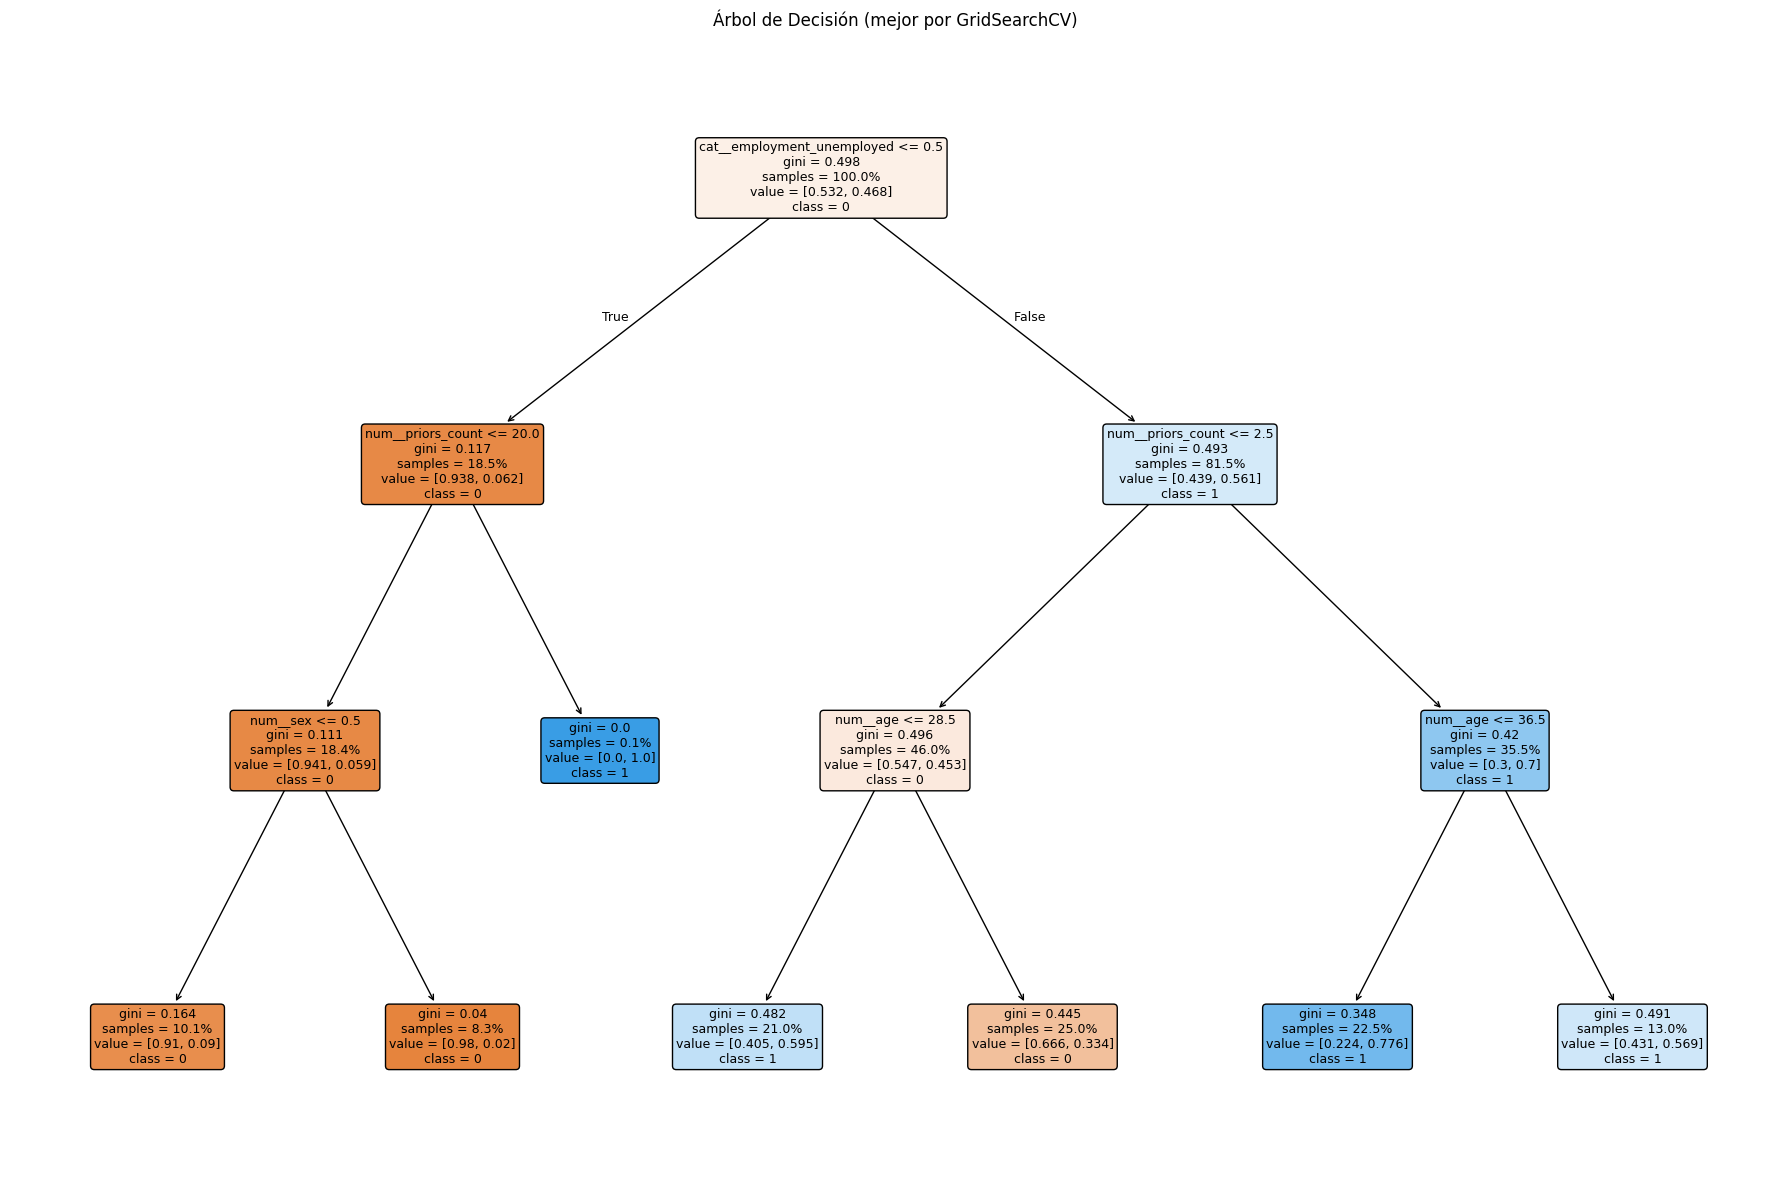
\includegraphics[width=0.92\linewidth]{figures/decision_tree_tunned_depth.png}
  \caption{Decision Tree (tuned), profundidad visualizada = 3.}
  \label{fig:tree-tuned}
\end{figure}











\subsection{Explicación global (resumen)}

El árbol ajustado concentra la decisión en pocas divisiones y umbrales sencillos, lo que facilita su lectura y comunicación. En la raíz aparece \texttt{employment\_unemployed}; a partir de ahí, \texttt{num\_priors\_count} y \texttt{age} modulan la predicción con cortes aproximados que se repiten en las ramas principales.

\paragraph{Tendencias clave.}
\begin{itemize}
  \item \textbf{Situación laboral}: si no está desempleado ($\leq 0.5$) la predicción suele inclinarse a clase 0; si está desempleado ($> 0.5$), el pronóstico depende sobre todo de antecedentes y edad.
  \item \textbf{Antecedentes} (\texttt{num\_priors\_count}): en personas empleadas, valores altos ($>20$) llevan a clase 1; en desempleados, el corte relevante baja (en torno a $2.5$).
  \item \textbf{Edad} (\texttt{age}): con pocos antecedentes, $\leq 28.5$ empuja a clase 1 y $>28.5$ a clase 0; con más antecedentes, incluso mayores de $\sim 36.5$ pueden seguir en clase 1.
  \item \textbf{Sexo}: aporta poco y solo ajusta la pureza en subramas concretas.
\end{itemize}

\paragraph{Reglas representativas (modelo ajustado).}
\vspace{-0.4em}
\begin{itemize}
  \item R1: \texttt{employment\_unemployed} $\leq 0.5$ $\land$ \texttt{num\_priors\_count} $\leq 20$ $\Rightarrow$ clase 0.
  \item R2: \texttt{employment\_unemployed} $\leq 0.5$ $\land$ \texttt{num\_priors\_count} $> 20$ $\Rightarrow$ clase 1.
  \item R3: \texttt{employment\_unemployed} $> 0.5$ $\land$ \texttt{num\_priors\_count} $\leq 2.5$: 
        si \texttt{age} $\leq 28.5$ $\Rightarrow$ clase 1; si \texttt{age} $> 28.5$ $\Rightarrow$ clase 0.
  \item R4: \texttt{employment\_unemployed} $> 0.5$ $\land$ \texttt{num\_priors\_count} $> 2.5$: 
        si \texttt{age} $\leq 36.5$ $\Rightarrow$ clase 1; si $> 36.5$ $\Rightarrow$ clase 1 (con menor pureza).
\end{itemize}

\paragraph{Comentario.}
El \texttt{GridSearch} no solo mejora ligeramente las métricas frente al baseline, sino que produce un árbol más \emph{compacto}: menos profundidad y menos reglas, por lo que se puede representar y recorrer con claridad.

\paragraph{Explicación local (instancia \#1535).}
A continuación se resume la instancia evaluada (valores originales, antes de OHE), la predicción del modelo 2 (tuned) y la ruta de decisión seguida dentro del árbol.

% --- Resumen de la fila (pre-OHE) ---
\begin{table}[h]
\centering
\caption{Instancia \#1535: valores originales.}
\label{tab:local-inst-1535}
\small
\begin{tabular}{@{}ll@{\hspace{1.8em}}ll@{}}
\toprule
\textbf{Variable} & \textbf{Valor} & \textbf{Variable} & \textbf{Valor} \\
\midrule
sex & 1 & juv\_misd\_count & 0 \\
age & 44 & juv\_other\_count & 0 \\
juv\_fel\_count & 0 & priors\_count & 2 \\
race\_African\texttt{-}American & 0 & race\_Caucasian & 1 \\
c\_charge\_degree\_F & 0 & c\_charge\_degree\_M & 1 \\
employment & \texttt{unemployed} & & \\
\bottomrule
\end{tabular}
\end{table}

% --- Predicción y hoja alcanzada ---
\begin{table}[h]
\centering
\caption{Predicción del modelo 2 para la instancia \#1535.}
\label{tab:local-pred-1535}
\small
\begin{tabular}{@{}lccc@{}}
\toprule
\textbf{Clase predicha} & \(\mathbf{P(y=0)}\) & \(\mathbf{P(y=1)}\) & \textbf{Hoja (id, n, gini)} \\
\midrule
0 (no recid) & 0.6658 & 0.3342 & id = 9,\; n = 739,\; 0.445 \\
\bottomrule
\end{tabular}
\end{table}

% --- Ruta de decisión (condiciones) ---
\begin{table}[h]
\centering
\caption{Ruta de decisión seguida (modelo 2).}
\label{tab:local-path-1535}
\small
\begin{tabular}{@{}cll@{}}
\toprule
\# & \textbf{Condición en el nodo} & \textbf{Rama} \\
\midrule
1 & \texttt{employment\_\_unemployed} \(> 0.5\) & Derecha \\
2 & \texttt{num\_\_priors\_count} \(\le 2.5\)   & Izquierda \\
3 & \texttt{num\_\_age} \(> 28.5\)              & Hoja (id=9) \\
\bottomrule
\end{tabular}
\end{table}

\textbf{Lectura rápida:} coincide con el patrón global —
\texttt{unemployed} $\land$ \texttt{priors} $\le 2.5$ y \texttt{age} $> 28.5$ $\Rightarrow$ \textbf{clase 0}.
Probabilidad estimada: $P(y=0)\approx 0.67$.
Nodo final con 739 casos; hay algo de mezcla de clases, así que la predicción es razonable pero no 100\% sólida.

